% L3b takeaway deck.
%
% THE DECK MIRRORS THE NOTEBOOK. Students use these slides as a note-taking
% companion while CHEME-5660-L3b-Lecture-LatticeModels-Equity-Price-Fall-2026.ipynb
% is shown live. The deck follows the notebook order and its real-world versus
% risk-neutral measure distinction.
%
% Notebook outline, and where each part lands in the deck:
%
%   (deck only)                             => title
%   Disclaimer and Risks          [last]    => slide 2 by instructor preference
%   Learning Objectives           [cell 0]  => Objectives for Today
%   Examples                                => Lectures and Examples
%   Binomial Lattice Model                  => figure, definition
%     Price Distribution                    => terminal prices, paths, nodes
%     Data-Driven Real World Parameter      => algorithm, caveats, recombination,
%       Estimation                             worked example
%     Model-Driven Risk-Neutral Probability => P versus Q, then no-arbitrage q
%                                              and replication value
%   Stylized Facts for Binomial Lattice     => overview frame
%     Return Distribution                   => Bernoulli transform, one-step
%                                              moments, binomial transform,
%                                              Heavy Tails
%     Temporal Dependence                   => Vanishing Autocorrelation, Nested
%                                              Windows, Volatility Clustering
%     (closing scorecard paragraph)         => What the Fixed Lattice Cannot Reproduce
%   Optional Advanced Material              => Optional Advanced Material
%   Summary                                 => Summary
%   Today?                                  => closing transition frame
%
% Two notes on the mapping. The lecture folds the P-versus-Q contrast into its
% risk-neutral subsection, so the deck's "Two Measures, Two Questions" frame
% opens that subsection rather than mirroring a separate heading. Probability of
% profit was dropped from the lecture and from this deck; POP is developed in
% week-10 (L10a POE/POP example, L10b composite-contract lecture).
%
% The lecture states the return-distribution and temporal-dependence results as
% theorems and moves their algebra to advanced/stylized-facts/. The deck keeps
% the result frames and does not derive them either.
\documentclass[aspectratio=169,11pt]{beamer}
\usepackage{vnslides}

\newcommand{\Pmeasure}{\mathbb{P}}
\newcommand{\Qmeasure}{\mathbb{Q}}

\title{\texorpdfstring{{\vnheavy L3b}}{L3b}: Equity-Price Lattices Under Real-World and Risk-Neutral Measures}
\subtitle{CHEME 5660 Cornell University}
\author{Copyright Jeffrey Varner 2026. All Rights Reserved}

\begin{document}

% ==== title ==================================================
\vntitlepage

% ==== disclaimer: intentional ordering exception =============
\begin{frame}{Disclaimer and Risks}
  \vspace{0.6em}
  \textbf{\ink{Training only.}} This content is for training and informational
  purposes only. The teaching team does not make, give, or endorse any offer or
  solicitation to buy or sell securities or derivative products, or provide
  investment or trading advice or strategy.

  \vspace{1.1em}
  \textbf{\ink{Risk.}} Trading involves risk and is generally not recommended for
  those with limited resources, experience, or a low risk tolerance. Past
  performance does not guarantee future success.

  \vspace{1.1em}
  \textbf{\ink{Responsibility.}} You are responsible for your investment decisions
  based on your financial circumstances, objectives, risk tolerance, and
  liquidity needs.
\end{frame}

% ==== objectives =============================================
\begin{frame}{Objectives for Today}
  \vspace{0.4em}
  Today we replace continuous price uncertainty with a finite lattice, derive
  its node distribution, and separate the probability used for forecasting from
  the one used for pricing.

  \vspace{0.9em}
  {\large\textbf{\ink{Today's concepts}}}
  \vspace{0.4em}
  \begin{itemize}\setlength{\itemsep}{0.5em}
    \item \hilite{Build a binomial lattice}: derive node prices and node
      probabilities from the up factor, down factor, horizon, and transition probability.
    \item \hilite{Separate probability measures}: explain why real-world
      probabilities support forecasting while risk-neutral probabilities support valuation.
    \item \hilite{Test model purpose}: identify which stylized facts the
      constant-parameter lattice reproduces and which its fixed parameters exclude.
  \end{itemize}
  \vspace{-0.4em}

  \slidenote{Companion notebook:}{\href{https://github.com/varnerlab/CHEME-5660-CourseRepository-Fall-2026}{L3b lecture notebook}}
\end{frame}

% ==== examples ===============================================
\begin{frame}{Lectures and Examples}
  \vspace{0.5em}
  {\normalsize\textbf{\ink{Lecture:}} \dimmed{CHEME-5660-L3b-Lecture-LatticeModels-Equity-Price-Fall-2026.ipynb}}

  \vspace{1.0em}
  {\normalsize\textbf{\ink{Example:}} \dimmed{CHEME-5660-L3b-LatticeModelSharePrice-RWPM-Example-Fall-2026.ipynb}}

  \vspace{0.9em}
  The example checks a textbook tree, estimates asymmetric move factors and a
  physical up probability from historical data, populates a recombining lattice,
  and compares its prediction bands with observed prices.

  \vspace{0.9em}
  The factors are \hilite{not} forced to satisfy $d=1/u$. That restriction is
  unnecessary for recombination.

  \slidenote{Link:}{\href{https://github.com/varnerlab/CHEME-5660-CourseRepository-Fall-2026.git}{https://github.com/varnerlab/CHEME-5660-CourseRepository-Fall-2026.git}}
\end{frame}

% ==== lattice schematic ======================================
\begin{frame}{A Recombining Price Lattice}
  \begin{center}
    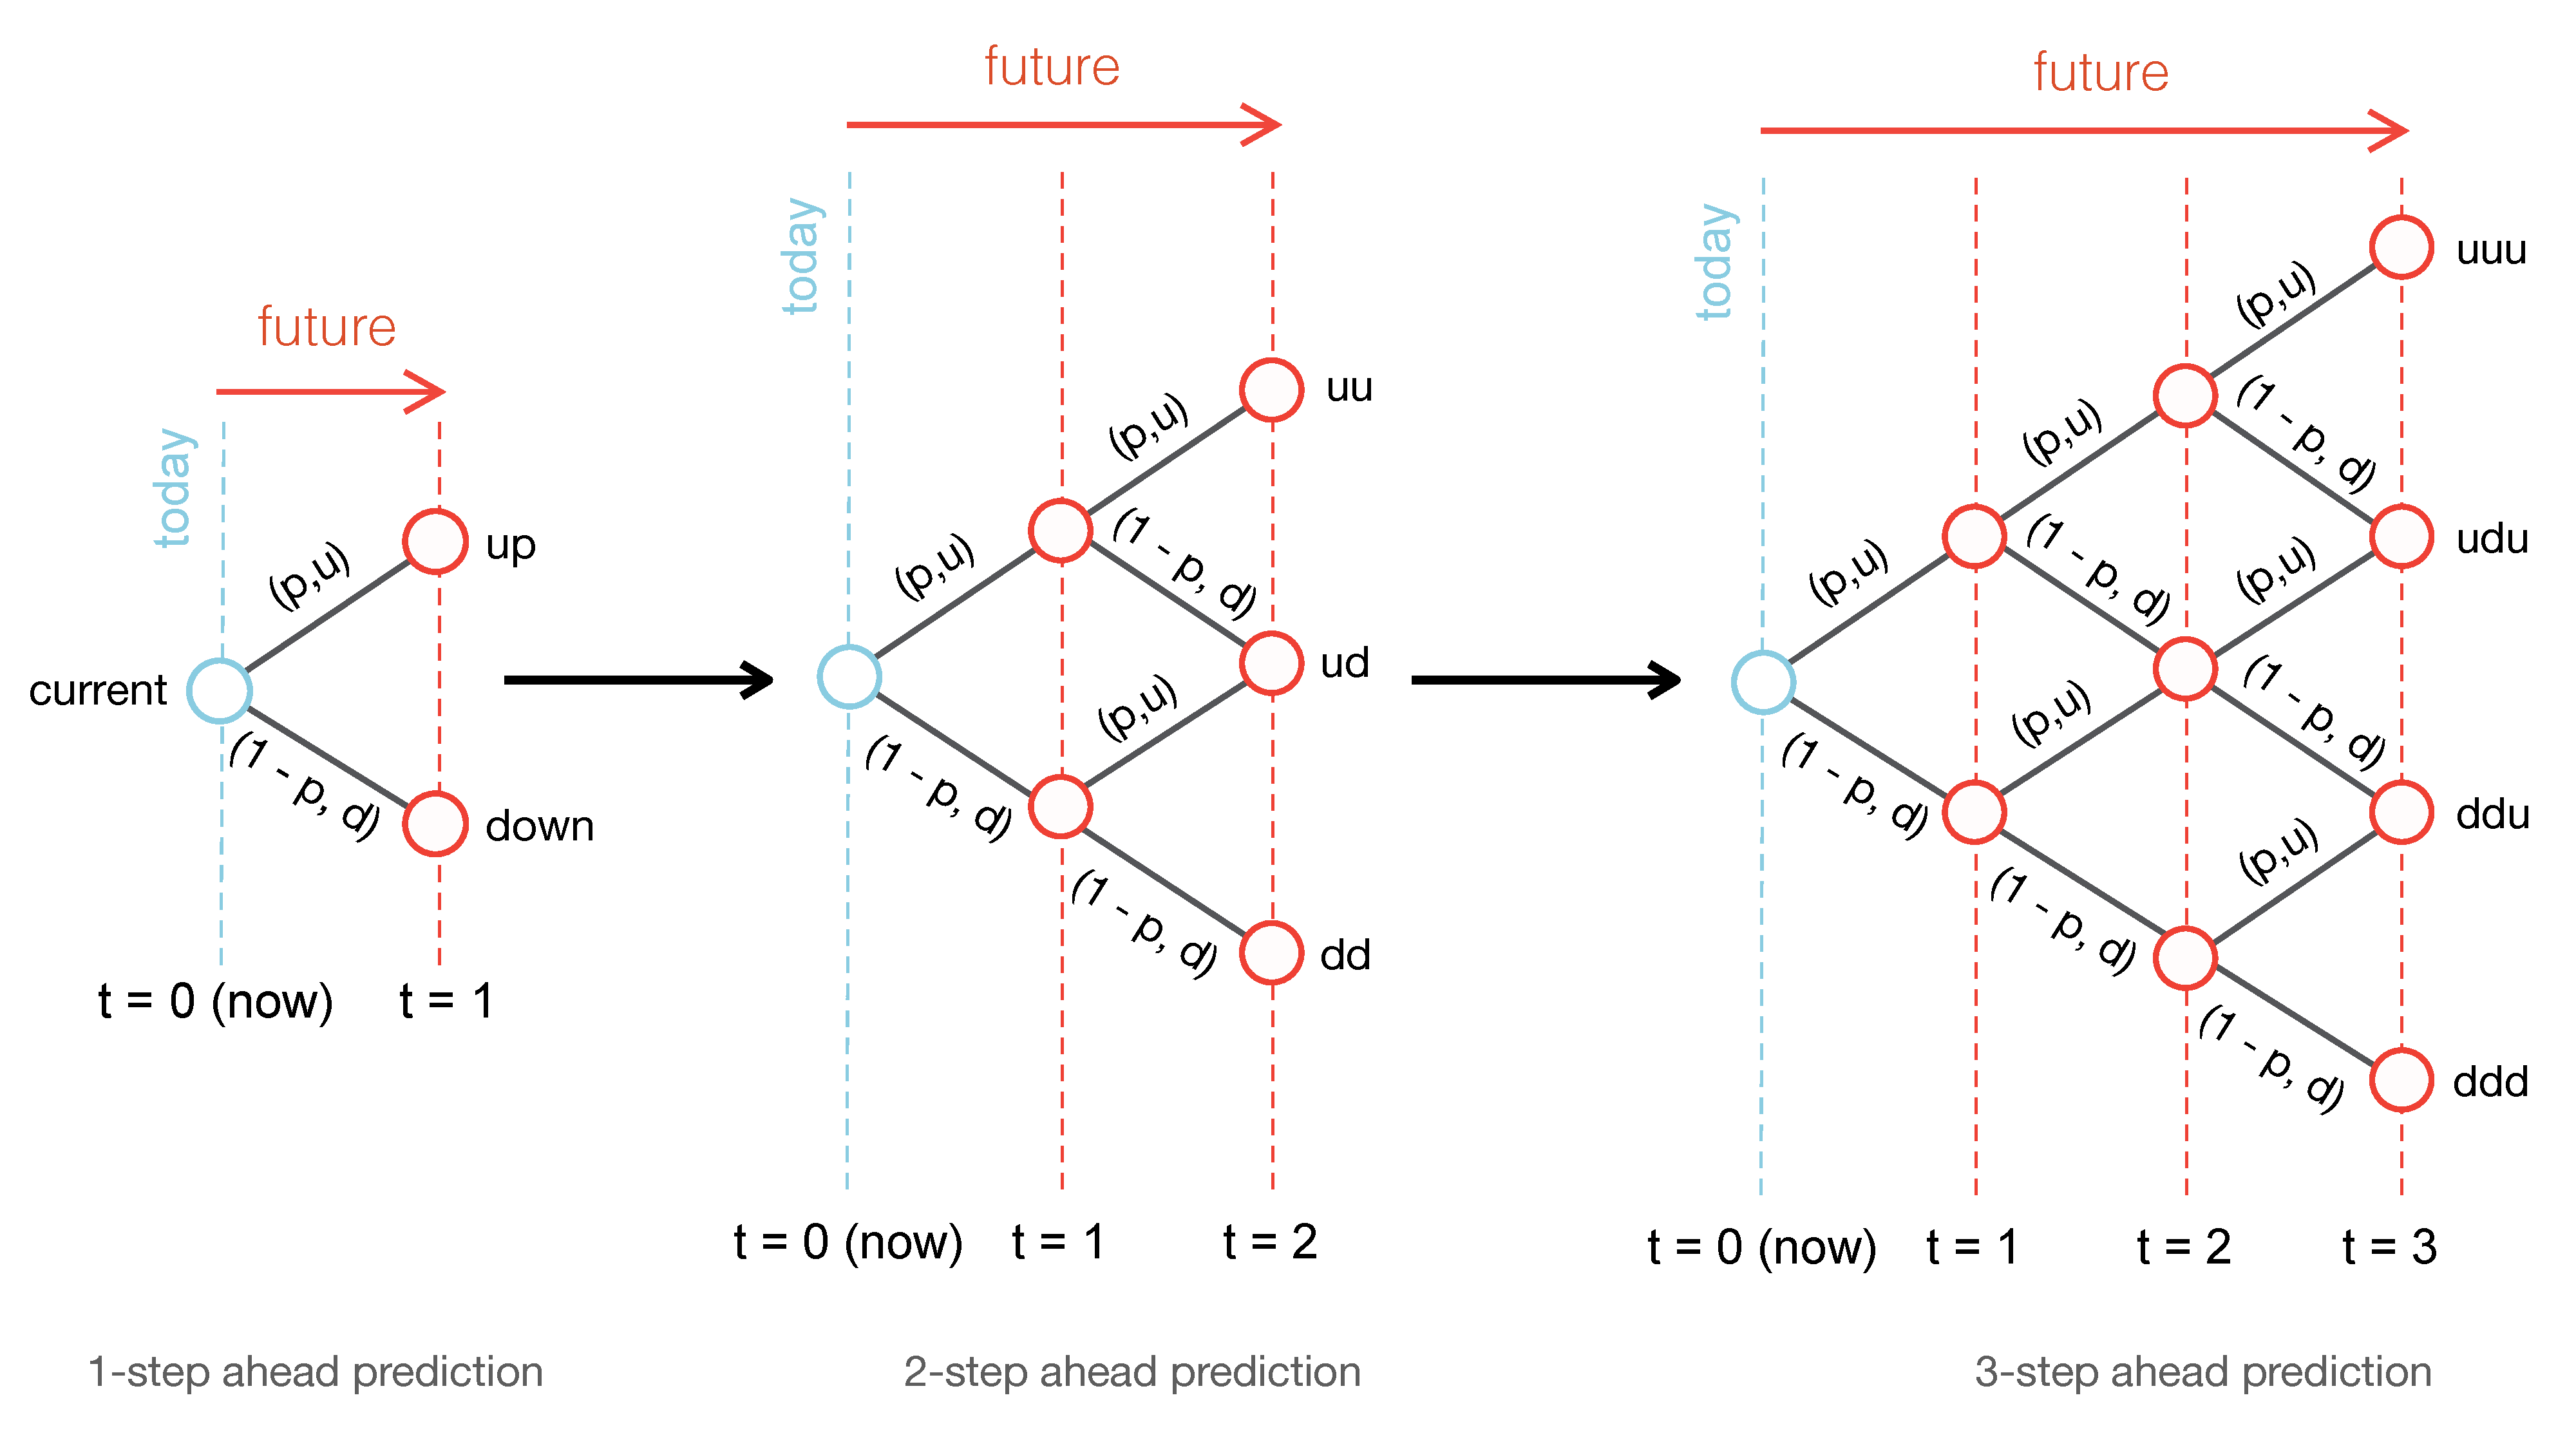
\includegraphics[height=0.77\textheight,keepaspectratio]{../figs/Fig-Lattice-Schematic.pdf}
  \end{center}
\end{frame}

% ==== lattice definition =====================================
\begin{frame}{Binomial Lattice Model}
  \vspace{0.2em}
  Let $S_0>0$ be today's ex-dividend share price. Over each step of length
  $\Delta t>0$ years, the price is multiplied by a constant \hilite{up factor}
  $u>0$ or a constant \hilite{down factor} $d>0$, with $d<u$.

  \vspace{0.5em}
  Under a real-world up probability $p\in[0,1]$, the one-step price is:
  \[
    S_1=
    \begin{cases}
      S_0u, & \text{with probability }p,\\
      S_0d, & \text{with probability }1-p.
    \end{cases}
  \]

  \vspace{0.3em}
  The fixed-parameter model assumes the same $u$, $d$, and $p$ at every node and
  independent move draws across steps. Level $t$ contains $t+1$ price states.

  \slidenote{Purpose:}{the lattice replaces a continuum of possible prices with a finite map whose probabilities and payoffs can be computed exactly.}
\end{frame}

% ==== terminal distribution ==================================
\begin{frame}{Terminal Prices and Their Distribution}
  Let $N$ be the number of independent steps, and let $K_N$ count the up moves.
  Under the real-world law, $K_N\sim\operatorname{Binomial}(N,p)$. Conditional on
  $K_N=k$, where $k\in\{0,\ldots,N\}$, the terminal price is:
  \[
    \underbrace{S_{N,k}=S_0u^kd^{N-k}}_{\text{\footnotesize terminal price}}.
  \]

  There are $\binom Nk$ paths with that count, and every such path has probability
  $p^k(1-p)^{N-k}$. The node probability is therefore:
  \[
    \underbrace{\Pmeasure(K_N=k)=\binom Nk p^k(1-p)^{N-k}}_{\text{\footnotesize probability of node }(N,k)}.
  \]

  The expected one-step gross return under this law is $pu+(1-p)d$.
\end{frame}

\begin{frame}{Paths Grow Exponentially, Terminal Nodes Linearly}
  \vspace{0.3em}
  After $N$ binary moves, the unmerged path tree contains $2^N$ paths to the
  terminal level. The recombining lattice contains only $N+1$ terminal price nodes.

  \vspace{0.8em}
  {\large\textbf{\ink{Why the compression is exact}}}
  \vspace{0.3em}
  \begin{itemize}\setlength{\itemsep}{0.6em}
    \item Every path with $k$ up moves and $N-k$ down moves reaches
      $S_0u^kd^{N-k}$.
    \item The binomial coefficient $\binom Nk$ records how many path orders merge
      into that node.
    \item Recombination preserves the terminal distribution while replacing path
      enumeration with one state per up-move count.
  \end{itemize}

  \vspace{0.5em}
  Backward valuation therefore walks nodes rather than paths.
\end{frame}

% ==== real-world estimation ==================================
\begin{frame}{\large Data-Driven Real World Parameter Estimation}
  Let $g_2,\ldots,g_T$ be historical growth rates sampled at interval
  $\Delta t>0$ years. Initialize an up-factor set $U$ and a down-factor set $D$.

  \vspace{0.4em}
  \begin{enumerate}\setlength{\itemsep}{0.4em}
    \item For every observation, place $e^{g_t\Delta t}$ in $U$ when $g_t>0$,
      in $D$ when $g_t<0$, and skip the factor when $g_t=0$.
    \item Estimate the conditional move magnitudes:
      \[
        \widehat u=\frac{1}{|U|}\sum_{v\in U}v,
        \qquad
        \widehat d=\frac{1}{|D|}\sum_{v\in D}v.
      \]
    \item Estimate the up probability by
      $\widehat p=|U|/(T-1)$, so zero-change days remain in the denominator.
  \end{enumerate}

  The sample must contain at least one up move and one down move.
\end{frame}

\begin{frame}{Historical Estimates Are Model Choices}
  \vspace{0.3em}
  The procedure turns historical observations into a \hilite{real-world forecast
  law}. It does not make the parameters timeless or uniquely correct.

  \vspace{0.7em}
  \begin{itemize}\setlength{\itemsep}{0.6em}
    \item Averaging positive and negative move factors compresses a continuous
      return distribution into two representative outcomes.
    \item Constant $u$, $d$, and $p$ discard serial dependence, changing
      volatility, and tail structure.
    \item Estimates inherit sampling error, the chosen observation window, data
      adjustments, and regime dependence.
    \item Validation must compare the entire out-of-sample distribution and path
      behavior with observations, not only the mean path.
  \end{itemize}

  \slidenote{Interpretation:}{$\widehat p$ is an estimated physical frequency, not a risk-neutral pricing probability.}
\end{frame}

\begin{frame}{\large Replacement, Recombination, and Reciprocal Moves}
  \vspace{0.2em}
  Three statements describe different features of the model.

  \vspace{0.5em}
  \begin{itemize}\setlength{\itemsep}{0.6em}
    \item \hilite{With replacement}: every step draws again from the same move
      set $\{u,d\}$. An up move does not remove the possibility of another up move.
    \item \hilite{Recombining}: move order does not change the final price because
      multiplication commutes:
      \[
        \underbrace{S_0ud}_{\text{up then down}}
        =\underbrace{S_0du}_{\text{down then up}}.
      \]
    \item \hilite{Reciprocal moves}: $d=1/u$, or $ud=1$, makes up and down
      increments symmetric in log space. It is an additional parameter choice.
  \end{itemize}

  \slidenote{Vocabulary:}{the unmerged path structure is a tree. After equal-price states merge, the lattice is a directed acyclic graph in the strict graph-theoretic sense.}
\end{frame}

\begin{frame}{Example: Asymmetric Moves Still Recombine}
  The companion notebook first checks $S_0=20$, $u=1.1$, $d=0.9$, and
  $p=0.6523$. These factors are asymmetric because:
  \[
    d=0.9\neq\frac{1}{1.1}\approx0.9091,
    \qquad
    ud=0.99\neq1.
  \]

  The two mixed paths still reach one shared node:
  \[
    \underbrace{20(1.1)(0.9)}_{\text{up then down}}
    =\underbrace{20(0.9)(1.1)}_{\text{down then up}}
    =19.8.
  \]

  Each ordered path has probability $p(1-p)$, so the recombined middle node has
  probability $2p(1-p)$. Reciprocal factors are unnecessary for both the shared
  price and the binomial node probability.

  \slidenote{Notebook:}{\dimmed{CHEME-5660-L3b-LatticeModelSharePrice-RWPM-Example-Fall-2026.ipynb}}
\end{frame}

% ==== probability measures ===================================
\begin{frame}{Two Measures, Two Questions}
  \vspace{0.2em}
  Two different probabilities are both called the probability of an up move.
  They answer different questions.

  \vspace{0.6em}
  \begin{columns}[T,onlytextwidth]
    \begin{column}{0.47\textwidth}
      {\large\textbf{\ink{Real-world $\Pmeasure$}}}
      \vspace{0.3em}
      \begin{itemize}\setlength{\itemsep}{0.45em}
        \item Up probability $p$ is estimated or modeled from data.
        \item Used for forecasts, scenarios, and risk measurement.
        \item Tested against out-of-sample distributions and paths.
      \end{itemize}
    \end{column}
    \begin{column}{0.47\textwidth}
      {\large\textbf{\ink{Risk-neutral $\Qmeasure$}}}
      \vspace{0.3em}
      \begin{itemize}\setlength{\itemsep}{0.45em}
        \item Up probability $q$ is implied by $u$, $d$, and the risk-free return.
        \item Used for no-arbitrage pricing and hedging.
        \item Tested by reproducing traded prices and excluding arbitrage.
      \end{itemize}
    \end{column}
  \end{columns}

  \vspace{0.7em}
  A pricing probability is generally \hilite{not} an empirical frequency.
\end{frame}

\begin{frame}{\large Model-Driven Risk-Neutral Probability}
  Let $R_f>0$ be the one-step risk-free gross return. For current equity price
  $S_0$ and next-step prices $S_0u$ and $S_0d$, absence of arbitrage requires:
  \[
    d<R_f<u.
  \]

  The unique risk-neutral up probability that makes the discounted share price
  a martingale is:
  \[
    S_0=\frac{qS_0u+(1-q)S_0d}{R_f},
    \qquad
    \underbrace{q=\frac{R_f-d}{u-d}}_{\text{\footnotesize risk-neutral probability}}.
  \]

  For a claim paying $H_u$ in the up state and $H_d$ in the down state, the same
  replication relation gives:
  \[
    V_0=\frac{qH_u+(1-q)H_d}{R_f}.
  \]

  This is an expectation under $\Qmeasure$, not a forecast of the realized payoff.
\end{frame}

% ==== stylized facts =========================================
\begin{frame}{Stylized Facts for Binomial Lattice Models}
  \vspace{0.3em}
  The lattice is our first model of equity-price dynamics. L3a gives three
  empirical patterns to test it against.

  \vspace{0.7em}
  \begin{itemize}\setlength{\itemsep}{0.6em}
    \item \hilite{Heavy tails}: large return magnitudes occur more often than a
      Gaussian model predicts.
    \item \hilite{Weak linear autocorrelation}: signed one-step returns usually
      carry little serial linear dependence.
    \item \hilite{Volatility clustering}: large movement magnitudes occur near
      other large movements, and calm observations near calm observations.
  \end{itemize}

  \vspace{0.5em}
  The fixed lattice matches the second pattern by assumption, but fails the first
  and third.

  \slidenote{Source:}{\href{https://doi.org/10.1080/713665670}{Cont (2001)}}
\end{frame}

\begin{frame}{Single-Step Growth Is a Bernoulli Transform}
  Let $X_j$ equal one for an up move and zero for a down move, with
  $X_j\stackrel{\mathrm{i.i.d.}}{\sim}\operatorname{Bernoulli}(p)$. The one-step
  price ratio is:
  \[
    \frac{S_j}{S_{j-1}}=u^{X_j}d^{1-X_j}
    =d\left(\frac ud\right)^{X_j}.
  \]

  Let $g_j$ be the continuously compounded growth rate over $\Delta t>0$ years.
  Taking logarithms gives:
  \[
    \underbrace{g_j=\frac{1}{\Delta t}
      \left[\log d+X_j\log\left(\frac ud\right)\right]}_{\text{\footnotesize two-point growth distribution}}.
  \]

  The lattice growth rate is therefore an affine transformation of a Bernoulli
  variable and takes only two possible values.
\end{frame}

\begin{frame}{One-Step Mean and Variance}
  Let $g_j$ be the two-point growth rate, with constant $u>d>0$, probability
  $p\in[0,1]$, and step length $\Delta t>0$. Its expected value is:
  \[
    \mathbb E[g_j]
    =\underbrace{\frac{p\log u+(1-p)\log d}{\Delta t}}_{\text{\footnotesize mean growth rate}}.
  \]

  Its variance is:
  \[
    \operatorname{Var}(g_j)
    =\underbrace{\frac{p(1-p)}{(\Delta t)^2}
      \left[\log\left(\frac ud\right)\right]^2}_{\text{\footnotesize fixed one-step variance}}.
  \]

  The variance is positive when $0<p<1$ and $u\neq d$. It vanishes at a
  degenerate probability or when the two moves coincide.
\end{frame}

\begin{frame}{Multi-Step Growth Is a Binomial Transform}
  Let $K_t\sim\operatorname{Binomial}(t,p)$ count the up moves in $t$ steps. The
  cumulative growth quantity $g_t=(1/\Delta t)\log(S_t/S_0)$ is:
  \[
    \underbrace{g_t=\frac{K_t\log(u/d)+t\log d}{\Delta t}}_{\text{\footnotesize binomial transform}}.
  \]

  Because $\mathbb E[K_t]=tp$ and $\operatorname{Var}(K_t)=tp(1-p)$:
  \[
    \mathbb E[g_t]=\frac{t}{\Delta t}\left[p\log u+(1-p)\log d\right],
  \]
  \[
    \operatorname{Var}(g_t)=\frac{tp(1-p)}{(\Delta t)^2}
      \left[\log\left(\frac ud\right)\right]^2.
  \]

  The corresponding cumulative log return is $r_t=(\Delta t)g_t=\log(S_t/S_0)$.
\end{frame}

\begin{frame}{Heavy Tails}
  \vspace{0.3em}
  \hilite{The fixed binomial lattice does not generate heavy-tailed growth.}

  \vspace{0.8em}
  \begin{itemize}\setlength{\itemsep}{0.65em}
    \item The one-step growth rate takes only two bounded values:
      $\log u/\Delta t$ and $\log d/\Delta t$.
    \item The multi-step growth quantity is an affine transformation of the
      binomial count $K_t$.
    \item When $0<p<1$ and $u\neq d$, the standardized binomial count converges
      to a Gaussian distribution as $t$ grows.
  \end{itemize}

  \vspace{0.6em}
  The model therefore predicts extreme moves less often than the heavy-tailed
  empirical distributions examined in L3a.
\end{frame}

\begin{frame}{Vanishing Autocorrelation}
  Let $g_j=b+aX_j$, where $a=\log(u/d)/\Delta t$,
  $b=\log d/\Delta t$, and the Bernoulli moves $X_j$ are independent. For every
  nonzero lag $\tau$:
  \[
    \operatorname{Cov}(g_j,g_{j+\tau})
    =a^2\operatorname{Cov}(X_j,X_{j+\tau})=0.
  \]

  Provided $0<p<1$ and $u\neq d$, the one-step variance is positive, so:
  \[
    \underbrace{\rho_g(\tau)=0\qquad(\tau\geq1)}_{\text{\footnotesize one-step autocorrelation}}.
  \]

  The lattice matches weak signed-return autocorrelation by construction. It does
  not discover that pattern from data: independence is an input assumption.
\end{frame}

\begin{frame}{Nested Windows Create Correlation}
  Let $g_t=aK_t+bt$ be cumulative growth from step $0$ through step $t$.
  The windows $0\rightarrow t$ and $0\rightarrow t+\tau$ share their first $t$
  moves, so their covariance is not zero:
  \[
    \operatorname{Cov}(g_t,g_{t+\tau})=a^2tp(1-p).
  \]

  Using the two variances gives:
  \[
    \underbrace{\rho(\tau)=\sqrt{\frac{t}{t+\tau}}}_{\text{\footnotesize nested-window correlation}}.
  \]

  This correlation is mechanical overlap, not predictability in one-step moves.
  Nonoverlapping $t$-step windows have zero correlation under the i.i.d. assumption.

  \slidenote{Careful:}{always state whether a return series uses overlapping or nonoverlapping windows before interpreting its autocorrelation.}
\end{frame}

\begin{frame}{Volatility Clustering}
  \vspace{0.3em}
  \hilite{The fixed binomial lattice does not generate volatility clustering.}

  \vspace{0.8em}
  Independence applies to the magnitudes, and the one-step variance is the same
  at every step:
  \[
    \operatorname{Cov}_{\Pmeasure}\!\left(|g_j|,|g_{j+\tau}|\right)=0,
    \qquad
    \operatorname{Var}_{\Pmeasure}(g_j)
    =\frac{p(1-p)}{(\Delta t)^2}
      \left[\log\!\left(\frac ud\right)\right]^2.
  \]

  \vspace{0.5em}
  Constant $u$, $d$, and $p$ create constant conditional volatility. The model
  cannot produce persistent high- and low-volatility regimes unless those
  parameters or the move law become state dependent.

  \slidenote{Connection to L3a:}{near-zero signed-return autocorrelation can coexist with strong dependence in squared returns, but the fixed lattice excludes that second dependence.}
\end{frame}

\begin{frame}{What the Fixed Lattice Cannot Reproduce}
  \vspace{0.3em}
  Because the lattice fixes its assumptions up front, we can say exactly what it
  captures and what it leaves out.

  \vspace{0.7em}
  \begin{itemize}\setlength{\itemsep}{0.6em}
    \item It captures positive prices, a complete finite distribution, weak
      one-step autocorrelation, and tractable backward valuation.
    \item It excludes continuous move sizes, heavy tails, volatility clustering,
      regime changes, and parameter uncertainty.
    \item A prediction band can have acceptable average coverage and still fail
      during exactly the extreme or high-volatility periods that matter most.
  \end{itemize}

  \vspace{0.6em}
  Use a lattice when the question is about states, trading rules, or replication.
  When the answer depends on rare moves or changing volatility, the move sizes or
  the parameters have to become state dependent.
\end{frame}

% ==== optional advanced material =============================
\begin{frame}{Optional Advanced Material}
  \vspace{0.3em}
  {\normalsize\textbf{\ink{Advanced 1:}} \dimmed{advanced/recombination/}\par
  \dimmed{CHEME-5660-L3b-Advanced-Recombination-ComputationalCost-Fall-2026.ipynb}}

  \vspace{0.5em}
  {\normalsize\textbf{\ink{Advanced 2:}} \dimmed{advanced/calibration/}\par
  \dimmed{CHEME-5660-L3b-Advanced-Bootstrap-LatticeCalibration-Fall-2026.ipynb}}

  \vspace{0.5em}
  {\normalsize\textbf{\ink{Advanced 3:}} \dimmed{advanced/stylized-facts/}\par
  \dimmed{CHEME-5660-L3b-Advanced-BinomialReturns-Derivations-Fall-2026.ipynb}}

  \vspace{0.5em}
  Optional, not prerequisites for L4a. The first compares the full path tree with
  its recombined lattice. The second bootstraps historical growth rates to measure
  the uncertainty in $(u,d,p)$. The third carries the algebra behind today's two
  theorems.
  \slidenote{Notebooks:}{\href{https://github.com/varnerlab/CHEME-5660-CourseRepository-Fall-2026/tree/main/lectures/week-3/L3b/advanced}{lectures/week-3/L3b/advanced}, also linked from the lecture notebook.}
\end{frame}

% ==== summary ================================================
\begin{frame}{Summary}
  This lecture built a recombining equity lattice, separated forecasting from
  pricing measures, and tested the fixed model against empirical return patterns.

  \vspace{0.45em}
  {\large\textbf{\ink{Key takeaways}}}
  \vspace{0.2em}
  \begin{itemize}\setlength{\itemsep}{0.35em}
    \item \textbf{\ink{Recombination is algebraic.}} A node depends on move
      counts because multiplication commutes. The constraint $ud=1$ is optional.
    \item \textbf{\ink{The measure follows the question.}} Real-world $p$
      supports forecasts and risk, while risk-neutral $q$ enforces no-arbitrage value.
    \item \textbf{\ink{The fixed lattice fails two of three tests.}} It
      matches weak one-step autocorrelation but misses heavy tails and volatility clustering.
  \end{itemize}

  \vspace{0.45em}
  The next step is to turn lattice states into explicit trading and valuation rules.
\end{frame}

% ==== closing ================================================
\transitionframe{That's a wrap. \hilite{Which lattice assumption would you relax
first, and what empirical pattern should the extension recover?}}

\end{document}
